\documentclass[tikz,border=2pt]{standalone}
\usepackage{amsmath}
\usetikzlibrary{arrows.meta}
\begin{document}
% Adding the odd values of 1:10 until the total exceeds 10: odd values are added,
% even values skipped with next; at x = 8 the total 16 > 10 triggers break; 9 and 10 are never visited.
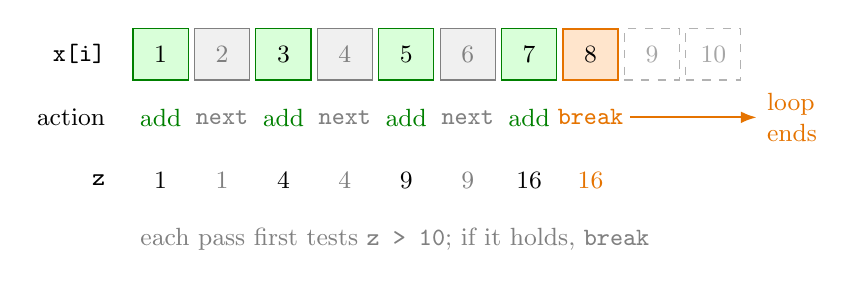
\begin{tikzpicture}[font=\small, >={Latex[length=2mm]},
  cell/.style={draw, minimum width=7mm, minimum height=6.5mm}]
  \node[anchor=east] at (0.2,0)    {\texttt{x[i]}};
  \node[anchor=east] at (0.2,-0.8) {action};
  \node[anchor=east] at (0.2,-1.6) {\texttt{z}};
  % added (odd)
  \foreach \k/\z in {1/1,3/4,5/9,7/16} {
    \node[cell, draw=green!50!black, fill=green!15] at (0.78*\k,0) {\k};
    \node[green!50!black] at (0.78*\k,-0.8) {add};
    \node at (0.78*\k,-1.6) {\z};
  }
  % skipped (even) with next
  \foreach \k/\z in {2/1,4/4,6/9} {
    \node[cell, draw=gray, fill=gray!12, text=gray] at (0.78*\k,0) {\k};
    \node[gray] at (0.78*\k,-0.8) {\texttt{next}};
    \node[gray] at (0.78*\k,-1.6) {\z};
  }
  % break
  \node[cell, draw=orange!90!black, fill=orange!20, thick] at (0.78*8,0) {8};
  \node[orange!90!black] at (0.78*8,-0.8) {\texttt{break}};
  \node[orange!90!black] at (0.78*8,-1.6) {16};
  % never visited
  \foreach \k in {9,10} {
    \node[cell, draw=gray!60, dashed, text=gray!70] at (0.78*\k,0) {\k};
  }
  \draw[->, thick, orange!90!black] (0.78*8+0.5,-0.8) -- (0.78*10+0.55,-0.8) node[right, align=left] {loop\\ends};
  \node[anchor=west, gray] at (0.4,-2.35) {each pass first tests \texttt{z > 10}; if it holds, \texttt{break}};
\end{tikzpicture}
\end{document}
